% -*- mode:flyspell; mode:latex -*-
% \documentclass[a4paper,twoside,11pt]{book}
\documentclass[12pt]{article}
\usepackage[latin1]{inputenc}
\usepackage[T1]{fontenc}
\usepackage[english]{babel}
\usepackage{graphicx}
\usepackage{float}


\usepackage{tikz}
\usepackage{[caption}
\usetikzlibrary{arrows}
\usetikzlibrary{decorations.markings}
\usetikzlibrary{decorations.pathmorphing}
% \usepackage[absolute,overlay]{textpos}
% \usepackage{onimage}

\usepackage{times}
\usepackage{graphics}

% \usepackage{subfigure}
% \usepackage{scalefnt}
% 
% \renewcommand\thesubfigure{\arabic{subfigure}}

\usepackage{amsmath}
\usepackage{hyperref}
\usepackage{hhline}
\usepackage{subfig}
\usepackage{color}
\usepackage[all]{hypcap}

% \usepackage[normalem]{ulem}  % for striking out
% \usepackage{fancyhdr}
% \pagestyle{fancy}
% \fancyhead[C]{}
% \fancyhead[L] {\it{Mu2e-doc-29670-v1.0} }
%%%%%%%%%%%%%%%%%%%%%%%%%%%%%%%%%%%%%%%%%%%%%%%%%%%%%%%%%%%%%%%%%%%%%%%%%%%%%%
% use natbib - biblatex not available on Mu2e interactive nodes
%%%%%%%%%%%%%%%%%%%%%%%%%%%%%%%%%%%%%%%%%%%%%%%%%%%%%%%%%%%%%%%%%%%%%%%%%%%%%%
\usepackage[square,sort,comma,numbers]{natbib}

% location of the .bib files: env var BIBINPUTS (~/library/bibliography)

% \usepackage[backend=biber, style=numeric-comp, sorting=ynt] {biblatex}
% \addbibresource{clfv.bib}

% \addbibresource{stntuple.bib}
% \addbibresource{mu2e_web.bib}
% \addbibresource{radiative_pion_capture.bib}

\graphicspath{{figures/}}
%%%%%%%%%%%%%%%%%%%%%%%%%%%%%%%%%%%%%%%%%%%%%%%%%%%%%%%%%%%%%%%%%%%%%%%%%%%%%%
% for portability, make sure all commands are included locally
%%%%%%%%%%%%%%%%%%%%%%%%%%%%%%%%%%%%%%%%%%%%%%%%%%%%%%%%%%%%%%%%%%%%%%%%%%%%%%
%\include{commands}
\newcommand {\Au}[1]     {\mbox{$\rm ^{#1}Au$}}                 % isotopes of gold
\newcommand {\mumemconv} {\mbox{$\mu^- A \rightarrow e^- A$}}
\newcommand {\mumepconv} {\mbox{$\mu^- A \rightarrow e^+ A$}}
\newcommand {\Pb}[1]     {\mbox{$\rm ^{#1}Pb$}}                 % isotopes of lead
%%%%%%%%%%%%%%%%%%%%%%%%%%%%%%%%%%%%%%%%%%%%%%%%%%%%%%%%%%%%%%%%%%%%%%%%%%%%%%
\begin{document}

\begin{titlepage}
  \begin{flushright}
    \bf {MU2E/PHYSICS/31019} \\
    version 1.0
    \today
  \end{flushright}

  \vspace{1cm}
  
  \begin{center}
    {\Large \bf What can be learned from the SINDRUM-II positron data on Au target} 
    
    \vspace{1cm}
    
    M.MacKenzie (NWU), P.Murat(FNAL)
    
    % \footnote{\texttt{Fermilab; e-mail: murat@fnal.gov}}
    \vspace{0.3cm}
    
    \vspace{0.8cm}                           
  \end{center}

  \begin{abstract}

    Positron data of the SINDRUM-II experiment on Au target have
    an interesting feature near the spectrum endpoint.
    We are trying to understand implications of that for the Mu2e
    search for \mumepconv\ .
    
  \end{abstract}

\end{titlepage}
% \frontmatter
% \chapter*{Abstract}
%
% \addcontentsline{toc}{chapter}{Abstract}
%
% \mainmatter
%
{\tableofcontents}

%%%%%%%%%%%%%%%%%%%%%%%%%%%%%%%%%%%%%%%%%%%%%%%%%%%%%%%%%%%%%%%%%%%%%%%%%%%%%%%
%\chapter{Calibration}
%%%%%%%%%%%%%%%%%%%%%%%%%%%%%%%%%%%%%%%%%%%%%%%%%%%%%%%%%%%%%%%%%%%%%%%%%%%%%%%
% \input{input_data}

%%%%%%%%%%%%%%%%%%%%%%%%%%%%%%%%%%%%%%%%%%%%%%%%%%%%%%%%%%%%%%%%%%%%%%%%%%%%%%%

\newpage
\section { Introduction}

The most stringent search limits for processes of \mumemconv\ and \mumepconv\
on nuclei come from the SINDRUM-II experiment \cite{sindrum_ii_Bertl2006}.

Br($\mu^- Au \rightarrow e^- Au) < 7·10^{-13}$ and

$Br(\mu^- Ti \rightarrow e^+ Ca) < 1.7·10^{-12}(GS)$

SINDRUM-II collected x2 muon stops on Au data as the 1997 Ti data,
and their '2006 paper also presented the positron data.
However no limit on \mumepconv\ has been published.

In this note we're trying to take a close look at the SINDRUM-II positron data
and understand their implications for the Mu2e search for \mumepconv\ .

\vspace{0.2in}
\begin{tikzpicture}
  \node[anchor=south west,inner sep=0] at (0,0.) {
    % \node[shift={(0 cm,0.cm)},inner sep=0,rotate={90}] at (0,0) {}
    \makebox[\textwidth][c] {
      \includegraphics[width=0.8\textwidth]{figures/png/sindrum_ii_2006_fig_11}
    }
  };
  % \node [text width=6cm, scale=0.8] at (4.5,6.4) {mu2e-18894 by Kevin Lynch and Jim Popp};
\end{tikzpicture}
\captionof{figure} {
  SINDRUM-II electron and positron spectra on Au target from 
}

Positron spectrum seems to have a bump near its high-momentum endpoint.
In this note we try to understand what are the implications of this bump
for the Mu2e search for the process of \mumepconv\ .

%%%%%%%%%%%%%%%%%%%%%%%%%%%%%%%%%%%%%%%%%%%%%%%%%%%%%%%%%%%%%%%%%%%%%%%%%%%%%% 
\newpage
\section { Approach}

We start from assuming that the dominant background in electron channel comes from DIO,
while the positron spectrum is dominated by the positrons from RMC photon conversions.
For \Au{197}, these assumptions hold better for positrons than for electrons:
in the vicinity of 90 MeV, RMC electrons also need to be taken into account.
There are more electrons than positrons (Compton scattering of the RMC photons),
so we just acknowledge the fact, but don't take any action, as the momentum distribution
of the electrons due to Compton scattering is not given in the 2006 paper.

SINDRUM-II used DIO spectrum on Pb tabulated in Watanabe'93 and corrected for the
difference of binding energies in \Au{197} and \Pb{208} for the DIO.

We use the electron spectrum to develop a simple parameterized model of
the SINDRUM-II detector response. The parameters include the momentum resolution,
assumed to be constant, and the overall reconstruction efficiency dependence on the 
track momentum.

We then use the response model to fit the positron spectrum below 88 MeV and
determine the RMC kMax. After that, we can predict the expected background
above 88 MeV and quantify the observed excess.

Finally we check if the observed excess is consistent with the signal expected from
\mumepconv\ on \Au{197}.

%%%%%%%%%%%%%%%%%%%%%%%%%%%%%%%%%%%%%%%%%%%%%%%%%%%%%%%%%%%%%%%%%%%%%%%%%%%%%%
%%%%%%%%%%%%%%%%%%%%%%%%%%%%%%%%%%%%%%%%%%%%%%%%%%%%%%%%%%%%%%%%%%%%%%%%%%%%%% 
\newpage
\section {Parameterization of the SINDRUM-II detector resolution}

placeholder
\begin{tikzpicture}
  \node[anchor=south west,inner sep=0] at (0,0.) {
    % \node[shift={(0 cm,0.cm)},inner sep=0,rotate={90}] at (0,0) {}
    \makebox[\textwidth][c] {
      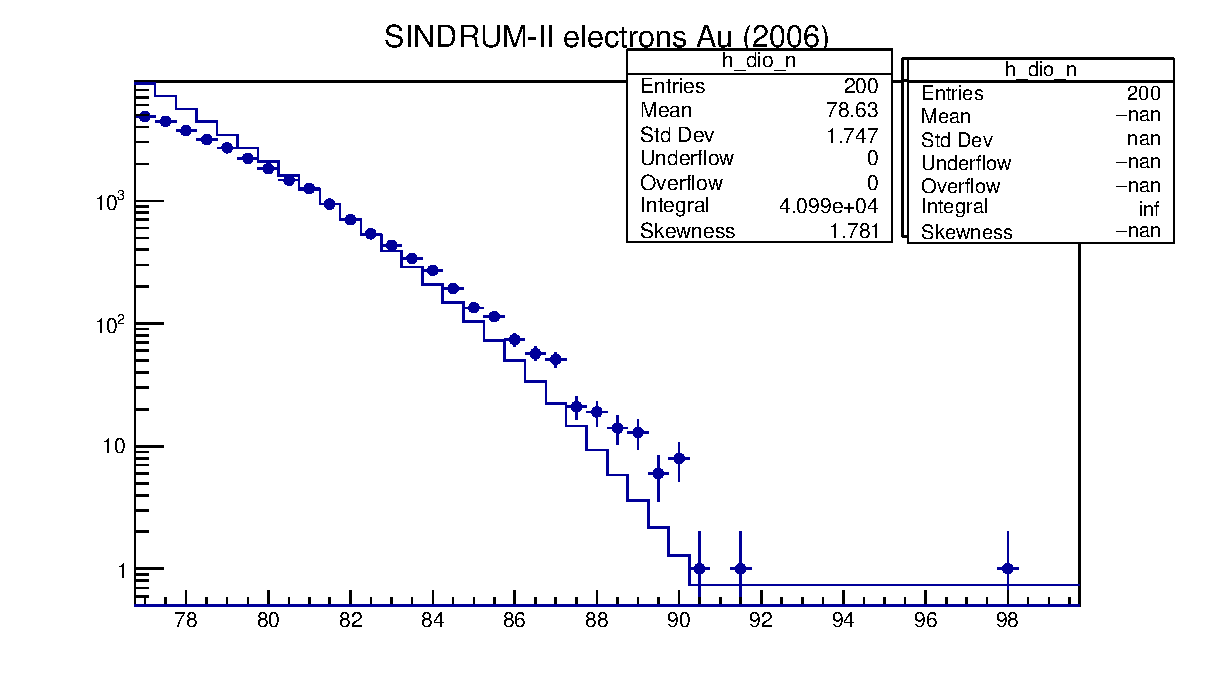
\includegraphics[width=0.99\textwidth]{figures/png/ana_step1_dio_normalized_above_80}
    }
  };
  % \node [text width=6cm, scale=0.8] at (4.5,6.4) {mu2e-18894 by Kevin Lynch and Jim Popp};
\end{tikzpicture}

placeholder
\begin{tikzpicture}
  \node[anchor=south west,inner sep=0] at (0,0.) {
    % \node[shift={(0 cm,0.cm)},inner sep=0,rotate={90}] at (0,0) {}
    \makebox[\textwidth][c] {
      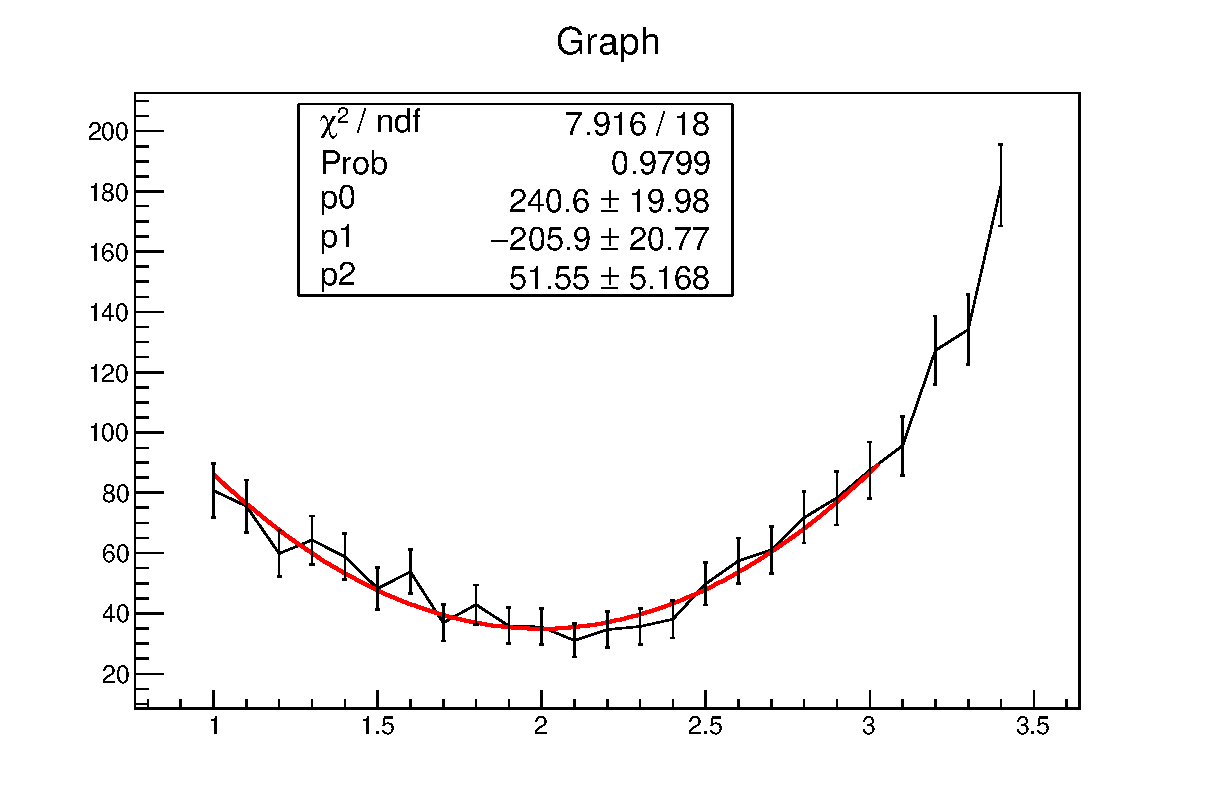
\includegraphics[width=0.99\textwidth]{figures/png/ana_step1_fit_sigma}
    }
  };
  % \node [text width=6cm, scale=0.8] at (4.5,6.4) {mu2e-18894 by Kevin Lynch and Jim Popp};
\end{tikzpicture}

%%%%%%%%%%%%%%%%%%%%%%%%%%%%%%%%%%%%%%%%%%%%%%%%%%%%%%%%%%%%%%%%%%%%%%%%%%%%%%
\newpage
\section {Tracking Efficiency Parameterization}

placeholder

\begin{tikzpicture}
  \node[anchor=south west,inner sep=0] at (0,0.) {
    % \node[shift={(0 cm,0.cm)},inner sep=0,rotate={90}] at (0,0) {}
    \makebox[\textwidth][c] {
      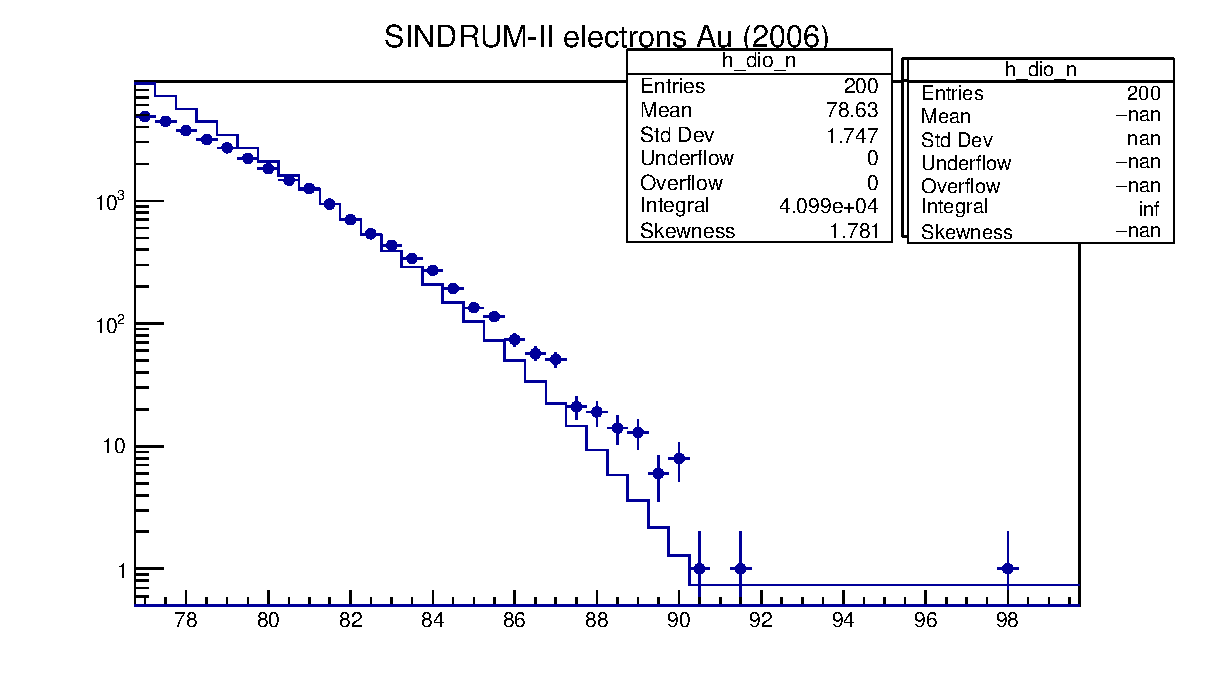
\includegraphics[width=0.99\textwidth]{figures/png/ana_step1_dio_normalized_above_80}
    }
  };
  % \node [text width=6cm, scale=0.8] at (4.5,6.4) {mu2e-18894 by Kevin Lynch and Jim Popp};
\end{tikzpicture}

Tuning the momentum resolution to get the right slope:

\begin{tikzpicture}
  \node[anchor=south west,inner sep=0] at (0,0.) {
    % \node[shift={(0 cm,0.cm)},inner sep=0,rotate={90}] at (0,0) {}
    \makebox[\textwidth][c] {
      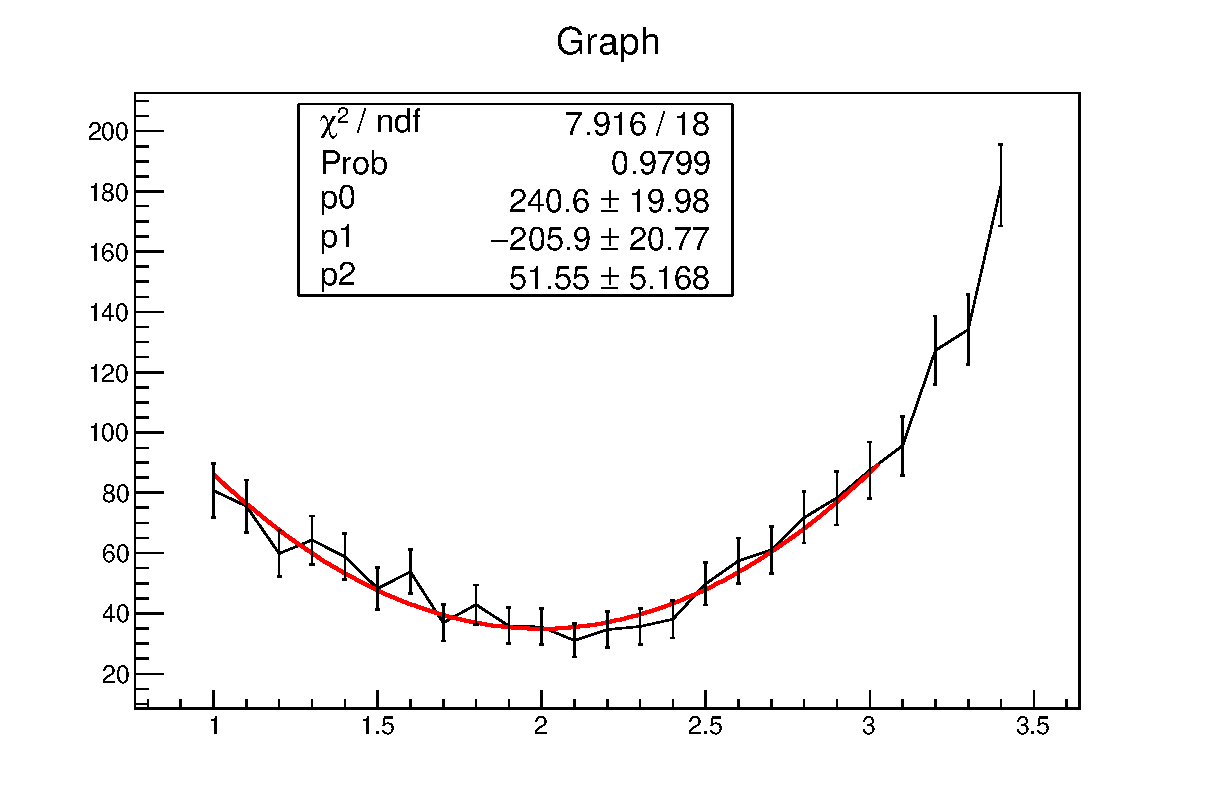
\includegraphics[width=0.99\textwidth]{figures/png/ana_step1_fit_sigma}
    }
  };
  % \node [text width=6cm, scale=0.8] at (4.5,6.4) {mu2e-18894 by Kevin Lynch and Jim Popp};
\end{tikzpicture}


Assume efficiency flat above 80 MeV/c, normalize MC to data in that region:

\begin{tikzpicture}
  \node[anchor=south west,inner sep=0] at (0,0.) {
    % \node[shift={(0 cm,0.cm)},inner sep=0,rotate={90}] at (0,0) {}
    \makebox[\textwidth][c] {
      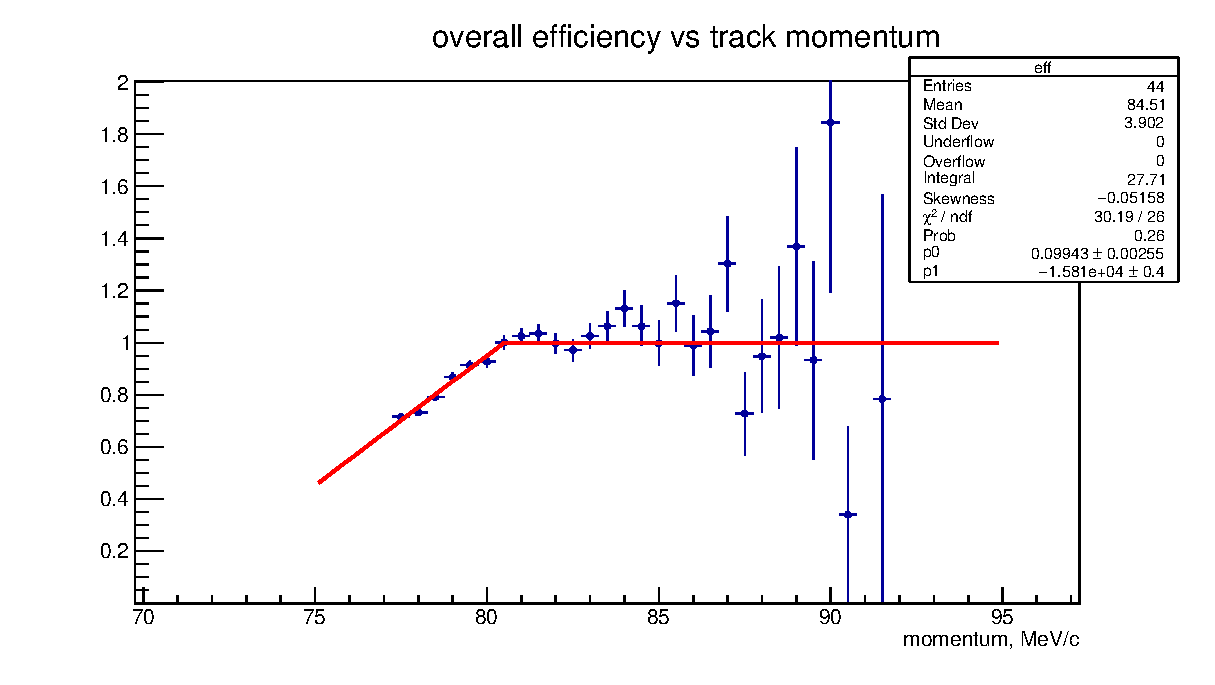
\includegraphics[width=0.99\textwidth]{figures/png/ana_step1_efficiency}
    }
  };
  % \node [text width=6cm, scale=0.8] at (4.5,6.4) {mu2e-18894 by Kevin Lynch and Jim Popp};
\end{tikzpicture}


Description of the electron spectrum after tuning:

\begin{tikzpicture}
  \node[anchor=south west,inner sep=0] at (0,0.) {
    % \node[shift={(0 cm,0.cm)},inner sep=0,rotate={90}] at (0,0) {}
    \makebox[\textwidth][c] {
      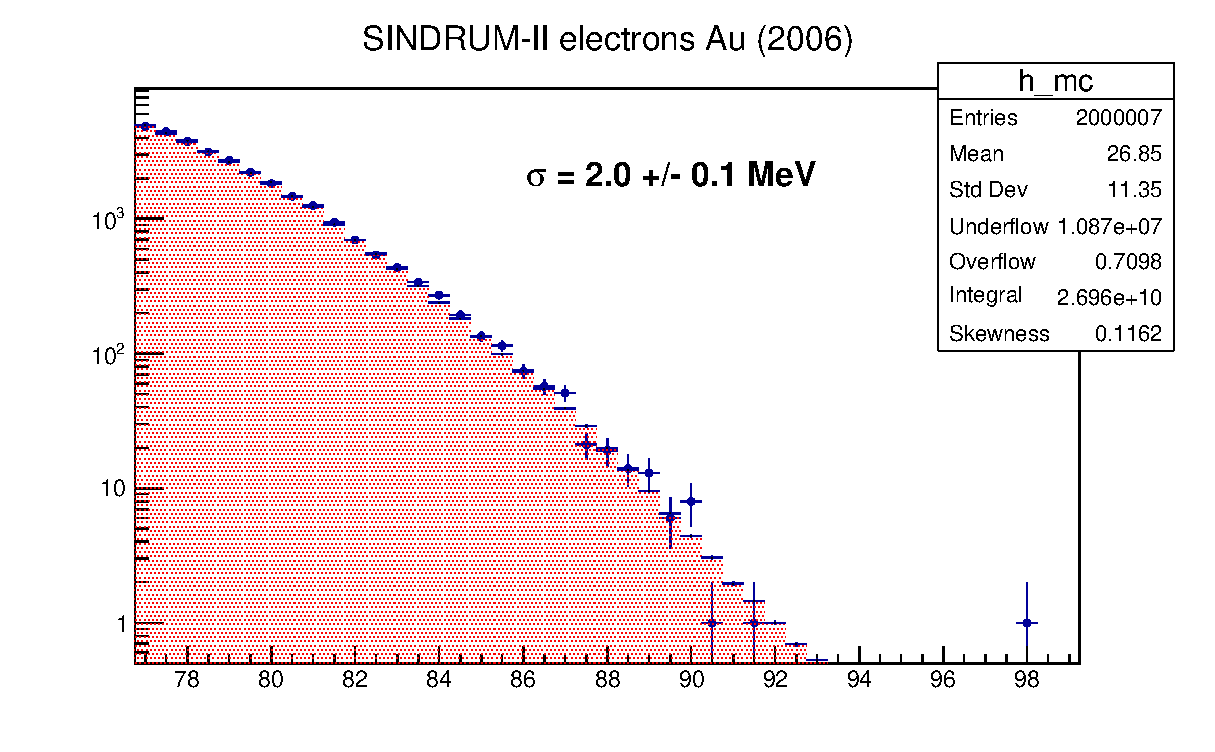
\includegraphics[width=0.99\textwidth]{figures/png/ana_step1_best_dio_fit}
    }
  };
  % \node [text width=6cm, scale=0.8] at (4.5,6.4) {mu2e-18894 by Kevin Lynch and Jim Popp};
\end{tikzpicture}

%%%%%%%%%%%%%%%%%%%%%%%%%%%%%%%%%%%%%%%%%%%%%%%%%%%%%%%%%%%%%%%%%%%%%%%%%%%%%% 
\newpage
\section {RMC spectrum and kMax Determination}

placeholder

%%% Local Variables:
%%% mode: latex
%%% TeX-master: t
%%% End:

%%%%%%%%%%%%%%%%%%%%%%%%%%%%%%%%%%%%%%%%%%%%%%%%%%%%%%%%%%%%%%%%%%%%%%%%%%%%%% 
\newpage
\section {SINDRUM-II momentum scale }

In \cite{sindrum_ii:Bertl2006}, the momentum scale has been calibrated using
the edge of the Michel spectrum from muon decays $\mu^+ \rightarrow e^+ \nu \bar{\nu}$
at rest. The calibration has been performed with the magnetic field reduced to about 50\%
of the nominal value. The reconstructed positron momentum distribution is shown
in Figure \ref{fig:sindrum_ii_fig_08_fit}.

{\bf replace electrons with positrons in the title below}

\vspace{0.1in}
\begin{tikzpicture}
  \node[anchor=south west,inner sep=0] at (0,0.) {
    % \node[shift={(0 cm,0.cm)},inner sep=0,rotate={90}] at (0,0) {}
    \makebox[\textwidth][c] {
      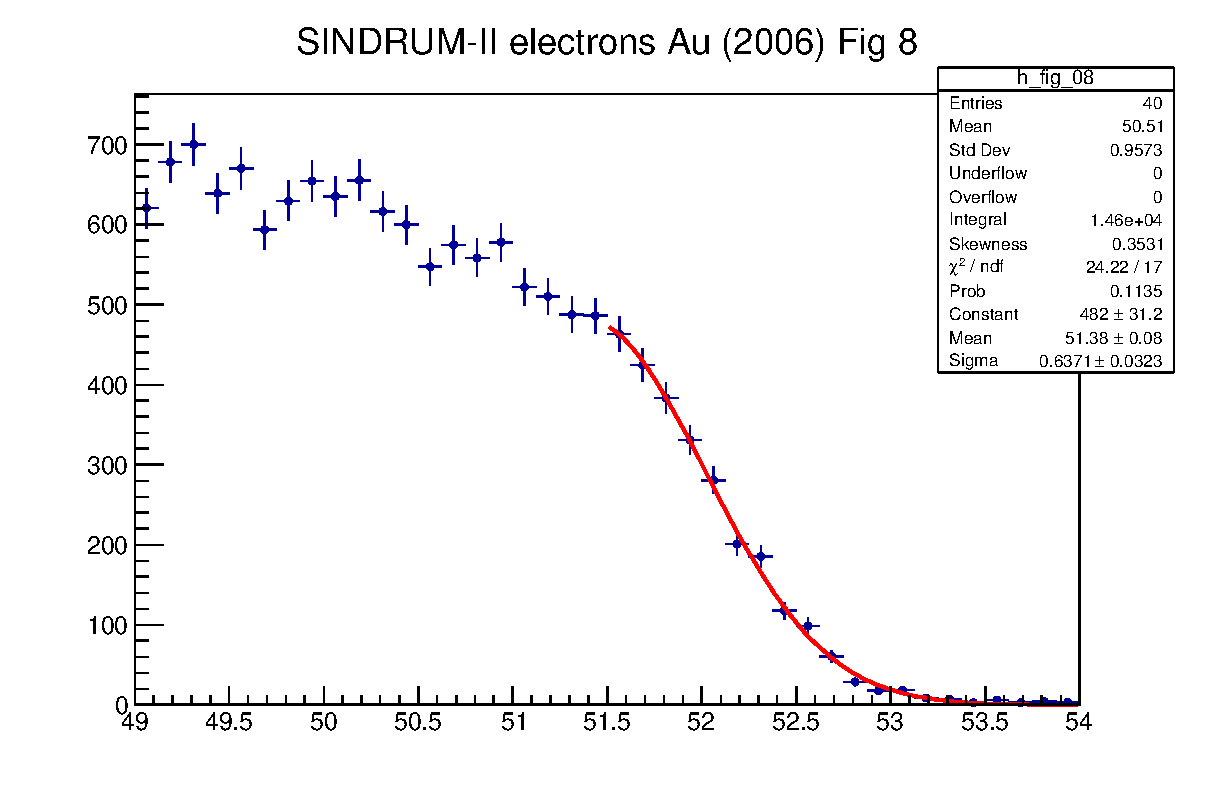
\includegraphics[width=0.99\textwidth]{figures/pdf/sindrum_ii_fig_08_fit}
    }
  };
  % \node [text width=6cm, scale=0.8] at (4.5,6.4) {mu2e-18894 by Kevin Lynch and Jim Popp};
\end{tikzpicture}
\captionof{figure} {
  \label{fig:sindrum_ii_fig_08_fit}
  Reconstructed momentum spectrum of positrons from $\mu^+ \rightarrow e^+ \nu \bar{\nu}$
  decays used in \cite{sindrum_ii:Bertl2006} for detector momentum calibration.
}
\vspace{0.1in}

Although radiative corrections modify the positron spectrum, as shown in Figure \ref{fig:mu2e_5645_fig_001_mue3_decay} their impact on the edge of the Michel spectrum
is fairly small, and the reconstructed position and shape of the edge depend primarily
on the energy losses and the momentum resolution.

\begin{tikzpicture}
  \node[anchor=south west,inner sep=0] at (0,0.) {
    % \node[shift={(0 cm,0.cm)},inner sep=0,rotate={90}] at (0,0) {}
    \makebox[\textwidth][c] {
      \includegraphics[width=0.99\textwidth]{figures/pdf/mu2e_5645_fig_001_mue3_decay}
    }
  };
  % \node [text width=6cm, scale=0.8] at (4.5,6.4) {mu2e-18894 by Kevin Lynch and Jim Popp};
\end{tikzpicture}
\captionof{figure} {
  \label{fig:mu2e_5645_fig_001_mue3_decay}
  Monte Carlo momentum spectrum of positrons from the $\mu^+ \rightarrow e^+ \nu \bar{\nu}$
  decay. Red: leading order, Blue: with radiative corrections taken into account.
}
\vspace{0.1in}

We expect the positron momentum referred to in the paper
to be the momentum in the first reconstructed point on the trajectory. As such, the
reconstructed Michel edge should be affected by the energy losses in front of the
tracker, their fluctuations, as well as the momentum resolution of the tracker.
According to \cite{sindrum_ii:Bertl2006}, the energy losses in front of the tracker are due to 
losses in the Au target (75 mg/cm$^2$) and the wall of the vacuum chamber (324 mg/cm$^2$),
main components of which are aluminum and carbon fiber.

To validate our understanding of the SINDRUM-II momentum calibration,
we simulate energy losses of positrons with initial momenta distributed uniformly
in the range [45,52.8] MeV/c in a structure consisting of the two layers described
above. The initial momentum distribution is shown
in Figure ~\ref{fig:sindrum_ii_michel_calibration} in red,
the positron momentum distribution on exit from the vacuum chamber wall is shown in blue.

{\bf Currently not shaded, need another iteration on the figure}

Shaded is the positron momentum distribution on exit convolved with
a Gaussian with $\sigma = 0.55$ MeV/c corresponding to the SINDRUM-II
momentum resolution of 1.3 MeV/c FWHM \cite{sindrum_ii:Kaulard1997_Thesis}.
The shaded distribution in Figure ~\ref{fig:sindrum_ii_michel_calibration}
double counts the fluctuations of energy losses, however the impact of double
counting is small and momentum edge smearing is dominated by the momentum
resolution of the tracker.

The fit of the high-momentum part of the smeared edge with the Gaussian returns
$\sigma = 0.63 \pm 0.03$ MeV/c, in good agreement with $\sigma = 0.64 \pm 0.03$ MeV/c
returned by the fit of the SINDRUM-II spectrum in Figure ~\ref{fig:sindrum_ii_fig_08_fit}.

\begin{figure} 
\begin{tikzpicture}
  \node[anchor=south west,inner sep=0] at (0,0.) {
    % \node[shift={(0 cm,0.cm)},inner sep=0,rotate={90}] at (0,0) {}
    \makebox[\textwidth][c] {
      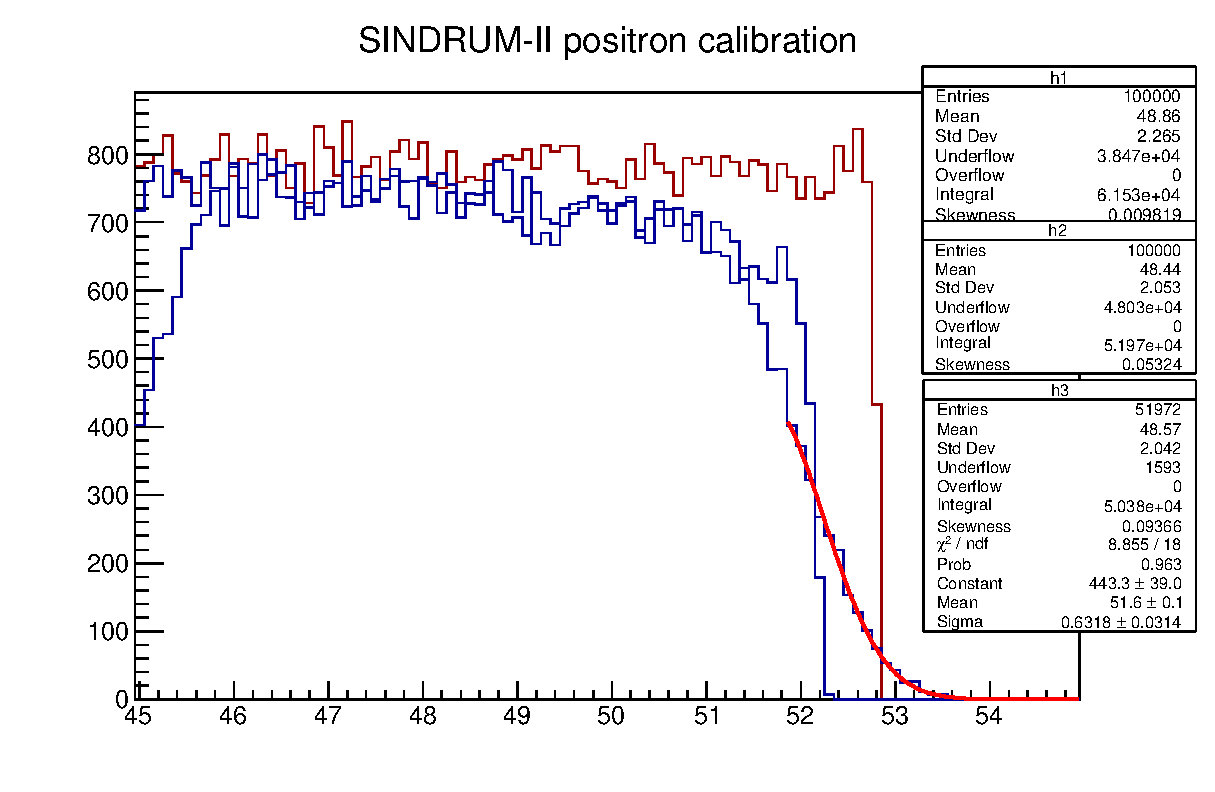
\includegraphics[width=0.99\textwidth]{figures/pdf/sindrum_ii_michel_calibration}
    }
  };
  % \node [text width=6cm, scale=0.8] at (4.5,6.4) {mu2e-18894 by Kevin Lynch and Jim Popp};
\end{tikzpicture}
% \caption{figure} {
\caption{
  \label{fig:sindrum_ii_michel_calibration}
  A flat spectrum with right edge 52.8 MeV is shown in red, the same spectrum convolved with 
  the expected energy losses is in blue, and then this distribution convolved with
  a Gaussian with $\sigma$ = 0.55 MeV is shaded.
}
% \vspace{0.1in}
\end{figure}

%%%%%%%%%%%%%%%%%%%%%%%%%%%%%%%%%%%%%%%%%%%%%%%%%%%%%%%%%%%%%%%%%%%%%%%%%%%%%% 

%%% Local Variables:
%%% mode: latex
%%% TeX-master: t
%%% End:

%%%%%%%%%%%%%%%%%%%%%%%%%%%%%%%%%%%%%%%%%%%%%%%%%%%%%%%%%%%%%%%%%%%%%%%%%%%%%% 
\newpage
\section {Events above 88 MeV and \mumepconv\ signal}

placeholder


%%%%%%%%%%%%%%%%%%%%%%%%%%%%%%%%%%%%%%%%%%%%%%%%%%%%%%%%%%%%%%%%%%%%%%%%%%%%%%
\subsection {Conversion Signal Resolution}

\begin{tikzpicture}
  \node[anchor=south west,inner sep=0] at (0,0.) {
    % \node[shift={(0 cm,0.cm)},inner sep=0,rotate={90}] at (0,0) {}
    \makebox[\textwidth][c] {
      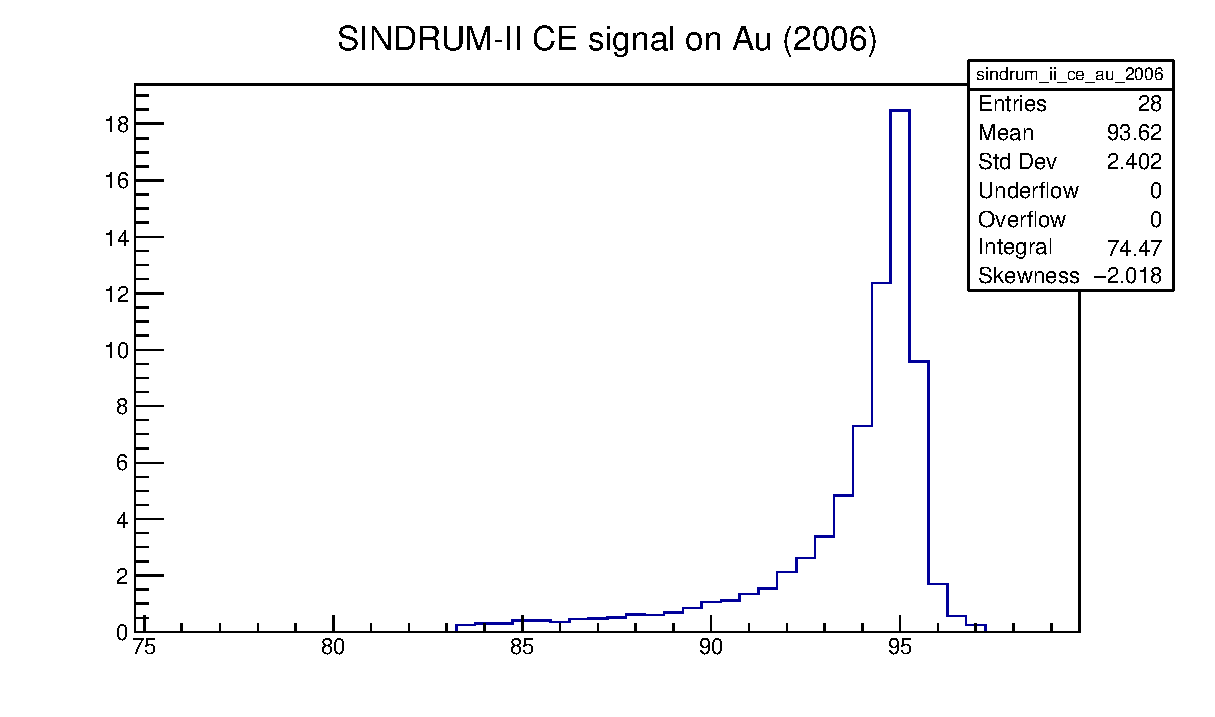
\includegraphics[width=0.99\textwidth]{figures/pdf/sindrum_ii_ce_signal}
    }
  };
  % \node [text width=6cm, scale=0.8] at (4.5,6.4) {mu2e-18894 by Kevin Lynch and Jim Popp};
\end{tikzpicture}


%%%%%%%%%%%%%%%%%%%%%%%%%%%%%%%%%%%%%%%%%%%%%%%%%%%%%%%%%%%%%%%%%%%%%%%%%%%%%%% 
\newpage
\section{ Summary }

What have we done...


%%%%%%%%%%%%%%%%%%%%%%%%%%%%%%%%%%%%%%%%%%%%%%%%%%%%%%%%%%%%%%%%%%%%%%%%%%%%%%% 
% \section{ Acknowledgements }
% 
% We want to thank ...
% 
%%%%%%%%%%%%%%%%%%%%%%%%%%%%%%%%%%%%%%%%%%%%%%%%%%%%%%%%%%%%%%%%%%%%%%%%%%%%%%
% \bibliography{radiative_muon_capture}
\bibliographystyle{unsrtnat}
\bibliography{clfv}
% \printbibliography
\end{document}


% ------------------------------------------------------------------------------
% templates
% ------------------------------------------------------------------------------
% Table ~\ref{table:summary} gives summary the numbers used in this study.
% 
% \hspace{-0.1in}
% \begin{table}[htbp]
%   \label{table:summary}
%   \begin{center} 
%     {\renewcommand{\arraystretch}{1.0}   % change 1.0 to 1.1 to increase the spacing between the table lines
%       \begin{tabular}{|c|c|c|c|}
%         \hline
%                             & default TS geometry & misaligned TS geometry   &  Ratio(default/misaligned)    \\ 
%         \hline
%         $N_{POT}$            &  $4.96 \cdot 10^6$  &    $5.00 \cdot 10^6$      &   0.992   \\ 
%         $N_{\mu}^{TS3u}$      &  65648              &     61354                 &   1.070   \\ 
%         $N_{\mu}^{TS5}$       &  28517              &     27351                 &   1.043   \\ 
%         $N_{\mu}^{ST}$        &  8868               &      8396                 &   1.056   \\ 
%         $N_{\mu}^{ST}/N_{POT}$ &  $1.79 \pm 0.02$    &    $1.68 \pm 0.02$        &   $1.065 \pm 0.03$        \\ 
%         \hline
%       \end{tabular}
%     }
%   \end{center}
%   \caption{
%     Muons rates at different points of the Mu2e beamline and stopping muon rates for nominal and 
%     misaligned TS geometries
%   }
%   % \vspace{0.5in}
% \end{table}
